% Part 2 chapter carrying sections 5-7 of "Dark Energy or Sector Tension?" (Mar 2026) line for line, corrected (sections 1-4: p2_09).
% Numbers: docs/verification/scripts/verify_sector_tension.py (+ _output.txt); mock: docs/verification/observations/TWO_RULER_DESI_TEST.md;
% Pantheon+ shape test: docs/verification/scripts/verify_dual_sector_validation.py. Errata SX1, SX3, SX4, SX7, SX8. Figure: figscripts/fig_p2_sector_s8.py.
\chapter{The phantom crossing and the two rulers}\label{ch:phantom}

\section*{The place}
The same horizon as Chapter~\ref{ch:sectortension}. Light measures distances on the photon ruler; matter grows and moves on the matter ruler. This
chapter takes the sector-assignment reading of DESI's phantom crossing, states it in full, and tests it.

\section{The sector-mixing argument}\label{sec:ph_mixing}
\conjecture\ The DESI preference for dark energy comes from joint fits of the $w_0w_a$CDM form to data sets that, under the informational term,
belong to two physically distinct sectors. In $\Lambda$CDM and in every standard single-fluid dark-energy model there is no such distinction: one
equation of state governs both the background distances and the growth of perturbations. Under the informational term the distinction follows from the
causal structure of spacetime. The sector assignment of the observables is:
\begin{itemize}
\item \emph{Photon ruler} ($\Lambda$CDM): BAO angular positions, the comoving distance $D_M(z)$ and the Hubble distance $D_H(z)$ in units of $r_d$, the
CMB acoustic scale $\theta_*$, and the relation between the lensing potential and the density ($\Sigma=1$). These are measured by light travelling on null
geodesics.
\item \emph{Matter ruler}: the growth rate $f\sigma_8$, peculiar velocities, the redshift-space-distortion parameter $\beta=f/b$, and the amplitude of
lensing, which follows the matter density. These are measured through the gravitational response of matter, $\mu<1$. The expansion rate that matter
measures is $\tilde H_m$ (Eq.~\ref{eq:st_hm}), giving $H_0^{\rm m}=67.16\sqrt{1+\beta_m}=72.26$ against the photon $67.16$ \calc.
\item \emph{Type Ia supernovae} are standard candles in galaxies, on timelike worldlines: the matter ruler. Their distances are read with light. With
the absolute magnitude free the supernova fit is exactly flat in $H_0$ (Chapter~\ref{ch:dsvalidation}).
\end{itemize}
\conjecture\ When a $w_0w_a$CDM model is fitted to both sectors at once it meets a definite conflict: the distances hold $H(z)$ to $\Lambda$CDM, while
the growth lies below what that $H(z)$ gives in a standard cosmology. The only freedom a single-fluid fit has to reproduce both a standard $H(z)$ and a
lower $f\sigma_8$ is a time-varying $w$: $w>-1$ recently, which lowers the integrated dark-energy contribution relative to $\Lambda$, and $w<-1$ earlier,
which compensates in the background. That is the phantom-crossing signature.

\section{The crossing redshift}
For $w(a)=w_0+w_a(1-a)$ the condition $w(a_{\rm cross})=-1$ gives $w_a(1-a_{\rm cross})=-(1+w_0)$, so
\begin{equation}
a_{\rm cross}=1+\frac{1+w_0}{w_a},\qquad z_{\rm cross}=\frac1{a_{\rm cross}}-1 .
\label{eq:ph_zcross}\end{equation}
\derived\ (checked with sympy). For the four DESI DR2 fits (Table~\ref{tab:st_dr2}) this gives:
\begin{table}[htbp]\centering\small
\caption{DESI DR2 $w_0w_a$CDM best fits~\cite{DESI2025} \observed, their crossing redshifts from Eq.~\eqref{eq:ph_zcross}, and the coupling and growth deficits
of the informational term at those redshifts \calc.}\label{tab:ph_cross}
\begin{tabular}{lccccc}\toprule
Data & $w_0$ & $w_a$ & $z_{\rm cross}$ & $1-\mu(z_{\rm cross})$ & $f\sigma_8$ deficit\\\midrule
DESI + CMB & $-0.42$ & $-1.75$ & 0.50 & 5.2\,\% & 1.36\,\%\\
DESI + CMB + Pantheon+ & $-0.838$ & $-0.62$ & 0.35 & 7.0\,\% & 1.91\,\%\\
DESI + CMB + Union3 & $-0.667$ & $-1.09$ & 0.44 & 5.9\,\% & 1.56\,\%\\
DESI + CMB + DES Y5 & $-0.752$ & $-0.86$ & 0.41 & 6.3\,\% & 1.69\,\%\\\midrule
informational term & $-1$ & $0$ & -- & 13.6\,\% today & 4.25\,\% today\\\bottomrule
\end{tabular}\end{table}
The crossing redshifts, $0.35$--$0.50$, lie in the range where the coupling deficit falls from about $7$ to $5\,\%$ and the growth-rate deficit from
about $1.9$ to $1.4\,\%$ (Fig.~\ref{fig:mu_evolution}b). \calc\ In the sector-mixing picture the crossing would appear where the disagreement between
matter and light is largest in relative terms, at low redshift where $E(a)$ is largest. \conjecture\ The coincidence of redshifts carries weight only if
the fits that produce the crossing contain growth data; the next section shows that they do not.

\section{The test}\label{sec:ph_test}
\begin{figure}[htbp]\centering
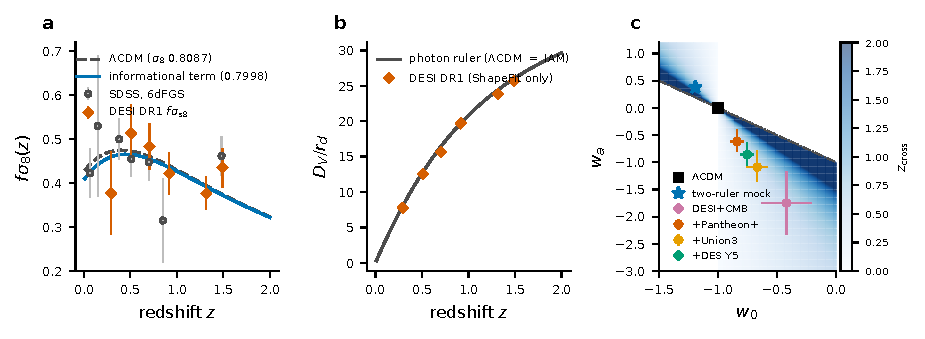
\includegraphics[width=\textwidth]{figures/part2/fig_sector_phantom.pdf}
\caption{Matter ruler, photon ruler and the $w_0$--$w_a$ plane. (a) $f\sigma_8(z)$: the informational term ($\sigma_8=0.7998$, $w=-1$, $\mu<1$) lies below $\Lambda$CDM ($\sigma_8=0.8087$) by at most $2.5\,\%$ in the DESI bins below $z=0.5$ \calc; diamonds, DESI DR1 ShapeFit-only $f\sigma_{s8}$ (Appendix~A of~\cite{DESI2024V}); circles, 6dFGS~\cite{Beutler2012} and SDSS~\cite{Alam2021} \observed. (b) $D_V/r_d$: the photon ruler, identical for the term and $\Lambda$CDM ($\Sigma=1$; Planck 2018, $r_d=147.09$\,Mpc) \calc, with the DESI DR1 ShapeFit-only measurements (Appendix~A of~\cite{DESI2024V}) \observed. (c) The DESI DR2 fits with the CMB and with each supernova sample~\cite{DESI2025} \observed; $\Lambda$CDM (square), which is the term's prediction for photon-ruler distances; the two-ruler mock (star: DESI DR2 BAO and the CMB on the photon ruler, 1,550 supernovae on $\tilde H_m$, magnitude free; $w_0=-1.19$, $w_a=+0.38$) \calc; shading, $z_{\rm cross}$ from Eq.~\eqref{eq:ph_zcross}; dash-dotted, the locus $w_0+w_a=-1$ on which $w=-1$ at $z\to\infty$.}\label{fig:sector_phantom}\label{fig:w0wa}
\end{figure}
Figure~\ref{fig:sector_phantom} sets the two sectors side by side. Panel (a) shows the matter ruler: the term's $f\sigma_8(z)$ lies below $\Lambda$CDM
by a margin that shrinks from $z=0$ to $z=2$, and the DESI DR1 and SDSS data are not yet precise enough to separate the two. Panel (b) shows the photon
ruler: the term's distances are those of $\Lambda$CDM at every redshift. The DESI ShapeFit-only distances scatter about the Planck $\Lambda$CDM curve,
most of all LRG2, whose isotropic dilation DESI reports $2$--$3\sigma$ low and reads as a statistical fluctuation~\cite{DESI2024V}; the scatter is common
to both models. Panel (c) shows the DESI DR2 fits, all displaced from $(-1,0)$ into the region $w_0>-1$, $w_a<0$. Three facts decide whether the
sector-mixing argument produces them.
\begin{enumerate}
\item The DR2 $w_0w_a$ fits use distances only: BAO, the CMB and supernovae. No growth data enter them, so mixing distances with growth cannot be what
moves them. \observed
\item Supernovae on the matter ruler with the shape $\tilde H_m(z)$ do mix two rulers in a distance-only fit. The mock (DESI DR2 BAO and the CMB on the
photon ruler, 1,550 supernovae on $\tilde H_m$, magnitude free) gives $w_0=-1.19$, $w_a=+0.38$: the opposite quadrant to DESI. In this form the
matter ruler shortens the low-redshift supernova distances, which a single fluid reads as more dark energy today. \calc
\item The real supernova data reject that shape. On Pantheon+ with full covariance~\cite{Brout2022}, applying $\tilde H_m$ to the supernova distances costs
$\Delta\chi^2=+23.6$; the supernova geometry is $\Lambda$CDM, and the matter ruler enters only through the calibration, which the free magnitude absorbs
(Chapter~\ref{ch:dsvalidation}). \calc
\end{enumerate}
So the informational term predicts photon-ruler distances that are $\Lambda$CDM, $w=-1$, and it does not produce DESI's preference. If that preference
holds, it is not this term. \prediction\ The mock is one implementation with simplified errors and no growth data; the full test runs the DESI
likelihoods with sector-dependent models, which the Level~2 CAMB code makes feasible (Section~\ref{sec:ph_limits}).

\section{Distinctive signatures}\label{sec:ph_signatures}
Three features separate the informational term from genuine dynamical dark energy.
\begin{itemize}
\item \emph{Scale independence.} The extra friction $\beta_mE(a)$ depends on time only, so the growth change is scale independent at linear order.
Dynamical dark energy and most modified-gravity theories give scale-dependent growth through a dark-energy sound horizon or a modified dispersion
relation. The DESI full-shape analysis contains scale information; testing whether a $w_0w_a$ preference survives when only a time-dependent growth
amplitude is varied would constrain this. \prediction
\item \emph{$\Sigma=1$ exactly.} The relation between the lensing potential and the density (weak-lensing convergence, CMB $C_\ell^{\phi\phi}$,
galaxy--galaxy lensing) is that of general relativity. Because $\delta_m$ is lower, the lensing power follows it down (CMB lensing $-0.08\,\%$) and the
statistic $E_G=\Omega_{m0}\Sigma/f$~\cite{Zhang2007EG} rises, by $1.8\,\%$ at $z=0.3$ and $3.6\,\%$ today (Table~\ref{tab:st_mu}). \calc\ Dark-energy models that
also lower growth generally change $\Sigma$ through the dark-energy perturbations, so their lensing and growth move together in a different ratio. The
ratio of growth to lensing measured in Euclid cross-correlations returns $f_{\rm IAM}$ if the term is right and differs if $\Sigma\neq1$. \prediction
\item \emph{The Hubble split.} The matter-sector rate $H_0^{\rm m}=67.16\sqrt{1+\beta_m}=72.26$ is $0.75\sigma$ from SH0ES ($73.04\pm1.04$); the photon-sector
$67.16\pm0.47$ is $0.37\sigma$ from Planck ($67.36\pm0.54$) \calc. A genuine $w\neq-1$ dark energy does not predict the size of the Hubble tension. The
$S_8$ shift and the $H_0$ split both follow from the one coupling $\beta_m$. \interp
\end{itemize}

\section{Discussion}
\paragraph{The consistency analyses.} \observed\ The two analyses of the DESI fits (\emph{MNRAS Lett.} 542, L24, 2025; arXiv:\allowbreak{}2504.04417)
examined the internal consistency of DESI DR1 $w_0w_a$CDM fits across data subsets, arguing that the preference may be driven by internal tensions in
the combined data rather than by a cosmological signal, and found that the DR2 constraints shift relative to DR1 in a way difficult to reconcile with a
stable dynamical dark energy. The informational term is a specific physical difference between data sets, growth against distances, that such
tensions could in principle reflect; for the distance-only DR2 fits it is not the source (Section~\ref{sec:ph_test}). \interp

\paragraph{Modified gravity.} $\mu<1$ with $\Sigma=1$ is unusual in the modified-gravity landscape~\cite{PogosianSilvestri2016}. \observed\ $f(R)$
gravity~\cite{HuSawicki2007} gives $\Sigma=1$ with $\mu$ between $1$ and $4/3$, enhanced growth. Horndeski scalar--tensor theories~\cite{BelliniSawicki2014}
can give $\mu<1$, generically with $\Sigma\neq1$, and $\mu-1$ and $\Sigma-1$ of opposite sign are strongly disfavoured~\cite{PogosianSilvestri2016}. The
normal branch of DGP gravity~\cite{DGP2000,KoyamaMaartens2006} gives $\mu>1$; the self-accelerating branch gives $\mu<1$ with $\Sigma=1$, but carries a
ghost~\cite{Koyama2007} and is in strong tension with growth and distance data~\cite{Fang2008}. Interacting dark-energy models can lower growth, but
through an interaction that also changes the background distances. \interp\ Under the informational term the combination $\mu<1$, $\Sigma=1$ is not a
parameter choice: it follows from the null-against-timelike decoherence argument, with no ghost and no free amplitude. \interp

\paragraph{Present and future precision.} The Level~1 chains with the amplitude free (Table~\ref{tab:lt_free}) give, for Planck + RSD, a posterior median
$\mu_0=+0.064$ with a one-sided $90\,\%$ lower bound $-0.204$: the prediction $\mu_0=-0.136$ lies inside the interval, and so does general relativity.
\fitted\ Present CMB and redshift-space-distortion data cannot separate the two at the predicted level. Euclid's forecast reach for the term's $\mu(z)$
runs from about $0.3\sigma$ with conservative scale cuts to about $7\sigma$ with the smallest scales modelled (Section~\ref{sec:lt_euclid}) \calc; the
lensing half of the signature, $\Sigma_0=0$, is the sharper test there.

\section{Limitations}\label{sec:ph_limits}
\begin{itemize}
\item \emph{Reduced growth calculation.} The growth equation (Eq.~\ref{eq:st_ode}) does not carry the Boltzmann hierarchy. The full prediction is the
Level~2 one, $\sigma_8=0.7998\pm0.0058$; the equation gives a $\sigma_8$ deficit of $0.78\,\%$ against the chains' $1.10\,\%$. The $f\sigma_8$ values of
Table~\ref{tab:st_fsig8} carry this caveat: adequate at present precision, they need the full calculation for comparisons below $1\,\%$.
\item \emph{The phantom-crossing test.} The two-ruler mock is not a likelihood analysis of the DESI pipeline. The full test runs the DESI full-shape and
BAO likelihoods with sector-dependent models, photon-sector and matter-sector observables each on its own expansion rate. This is feasible with the
Level~2 CAMB code and needs a dedicated analysis of the DESI data vectors. \openprob
\item \emph{$S_8$ at fixed $\Omega_m$.} The lensing comparison uses survey $S_8$ values from $\Lambda$CDM analyses. Under the two-sector reading the
matter-sector $\Omega_m$ that a weak-lensing survey measures would be lower than the CMB value (Chapter~\ref{ch:virial_tests}); a rigorous comparison
reprocesses the survey likelihoods with the modified growth. \interp\ \openprob\ Table~\ref{tab:st_s8} compares like with like: each chain's $S_8$
with the published survey values.
\item \emph{Correlations between bins.} The DESI DR1 values of Table~\ref{tab:st_fsig8} are treated as independent, and the growth entry is
$f\sigma_{s8}$, which depends on the template. A $\chi^2$ analysis uses the published covariance of the full data vectors~\cite{DESI2024V}; the pulls
and diagonal $\chi^2$ here are indicative.
\end{itemize}

\section{Conclusions}
The informational term has been confronted with the DESI DR1 full-shape growth rates in six bins, the DESI DR1 distances, the weak-lensing values
from KiDS, DES Y3 and HSC Y3, and the DESI DR2 $w_0w_a$ fits. The findings:
\begin{enumerate}
\item Its $f\sigma_8(z)$ is consistent with the DESI DR1 ShapeFit data in all six bins ($0.295\le z_{\rm eff}\le1.491$), pulls $-0.88$ to $+1.40$, and so
is $\Lambda$CDM. The growth-rate deficit is $2.2\,\%$ at the lowest DESI bin and below $0.2\,\%$ above $z\approx1.3$. \calc
\item Its distances are $\Lambda$CDM at every DESI redshift, as $\Sigma=1$ from the null-worldline argument requires. \prediction
\item Its $\sigma_8=0.7998\pm0.0058$ (Level~2) agrees with the 2025 joint lensing value at $0.1\sigma$; its $S_8=0.822$ lies $0.4\sigma$ above the
completed KiDS survey and $1.4$--$2.5\sigma$ above KiDS-1000, DES Y3 and HSC Y3. \calc
\item The DESI DR2 crossing redshifts, $0.35$--$0.50$, fall where the coupling deficit is $5$--$7\,\%$, but the DR2 fits contain no growth data, the
matter-ruler supernova shape moves a fit to the opposite quadrant, and Pantheon+ rejects that shape. Under the term $w\equiv-1$, and the term does not
produce DESI's preference. \calc
\item Under the full Planck 2018 likelihood the term reproduces the CMB as well as $\Lambda$CDM with no added parameter ($\Delta\chi^2=+0.54$ at the best points,
eighteen converged chains, $R-1<0.01$), with $\beta_m=0.15765$ fixed and the posterior $\Omega_m/2$ consistent with it at $0.2\sigma$. \measured
\end{enumerate}
Two near-term tests:
\begin{itemize}
\item \emph{The $\mu$--$\Sigma$ measurement.} $\mu_0=-0.136$ with $\Sigma_0=0$ exactly; the reach of Euclid is in Section~\ref{sec:lt_euclid}. The
simultaneous constraint $\Sigma_0=0$, from CMB lensing and weak-lensing convergence ratios, is needed to confirm the null-sector reading. $\mu_0$
consistent with zero at the precision that separates the two falsifies the term. \prediction
\item \emph{The $f\sigma_8(z)$ shape.} A specific curved deficit set by $E(a)=\exp(1-1/a)$, separable from a constant rescaling and from the growth
history of a $w\neq-1$ model: $3.1\,\%$ at $z=0.15$, $1.9\,\%$ at $0.35$, $0.9\,\%$ at $0.65$, $0.4\,\%$ at $1.05$ and $0.1\,\%$ at $1.55$. At $1\,\%$
per bin over fifteen bins of width $0.1$ in $0.1<z<1.6$, a precision the completed DESI survey is designed to approach, the shape is $5.0\sigma$ from
$\Lambda$CDM \calc. \prediction
\end{itemize}

The tests above are ready to run: measure $\mu$ and $\Sigma$ together, and check the $f\sigma_8$ shape bin by bin. A cosmologist with the public chains can run both and see directly which way the result falls.

\section{Status}
The sector assignment and the growth and lensing signatures are predictions of the informational term, with $\mu_0=-0.136$ \prediction; the $H_0$
split, $67.16$ and $72.26$, follows from the Level~2 chains \calc. Calculated here: the growth deficits at the DESI redshifts are $0.1$--$2.2\,\%$,
below current errors, and the DESI phantom crossing is not produced by the informational term. \calc\ Scripts, chains and the modified Fortran source
(\texttt{equations\_iam\_level2.f90}) are in the repository.
